\documentclass[a4paper,11pt]{scrartcl}

\usepackage[margin=1in]{geometry}
\usepackage[scaled]{helvet}
\usepackage[T1]{fontenc}
\usepackage[utf8]{inputenc}
\usepackage{amsmath}
\usepackage{mathptmx}
\usepackage{courier}
\usepackage{graphicx}
\usepackage{ulem}
\usepackage{bookmark}
\usepackage{paralist}
\usepackage{ngerman}
\usepackage{fancyhdr}
\usepackage{float}
\usepackage{array}

\graphicspath{ {../img/} }
\renewcommand\familydefault{\sfdefault}

\pagestyle{fancy}
\fancyhf{}
\renewcommand{\headrulewidth}{0pt}
\fancyfoot[C]{
\includegraphics[width=\textwidth]{Polygon_gruen}\\ \thepage}

\rhead{
\includegraphics[width=\textwidth]{LogoHeader}}
\setlength\headheight{30pt}
\setlength\footskip{15pt}

\begin{document}
\renewcommand*{\arraystretch}{1.2}
\pagenumbering{gobble}
\begin{titlepage}
    \begin{center}
        \vspace*{1cm}\Huge
        \textbf{Anforderungsanalyse}\par                
        \vspace{0.5cm}\LARGE        
        Software Engineering II\par           
        \vspace{2cm}
        
\includegraphics[width=0.5\textwidth]{OptimaLogo_long}\par   
        \vspace{1cm}
        \textbf{Projekttitel: BonoboBoard}\par        
        \vfill\Large   
        Jakob Hutschenreiter (1419081)\\Jiesen Wang (9839152)\\Nick Kramer (3122448)\\Patrick Küsters (2598689)\\Peter Moritz Hinkel (2783930)\par
        %\vspace{2cm}  
        %
\includegraphics[width=0.5\textwidth]{Bonobo_Logo}\par        
        \vspace{2cm}
        DHBW Mannheim\\
        \today     
    \end{center}
\end{titlepage}

\section*{Änderungshistorie}
\begin{table}[h]
	\begin{tabular}{@{} p{20mm} p{25mm} p{40mm} p{75mm}}
		\textbf{Revision} & \textbf{Datum} & \textbf{Autor(en)} & \textbf{Beschreibung}\\
		1.0 & 31.01.2022 & NK|PK & A: 1.1, 1.2, 1.3\\
		1.1 & 31.01.2022 & JW & A: 1.3, C: 1.1, 1.2, 1.3\\
		1.2 & 04.02.2022 & JW|NK|derPeder|PK & A: 2.1, 2.2, 3 \\
	\end{tabular}
\end{table}
\noindent
Abkürzungen: Hinzugefügt/Added (A), Änderung/Changed (C), Löschung/Deleted (D)
\vspace{2cm}
\tableofcontents
\newpage
\pagenumbering{arabic}

		%------------------------------------------------------------
		%-----  -----  ----- Begin actual content -----  -----  -----
		%------------------------------------------------------------


\section{Einleitung}
	\subsection{Motivation} % Motivation, Thema, Ziel
BonoboBoard ist eine kostenfreie Webanwendung für alle Studierenden der DHBW Mannheim, die statt vieler unabhängiger Websites eine einzige Übersicht aller auf die Hochschule bezogenen Inhalte erhalten wollen.\\
Es stellt Funktionen bereit, die alle relevanten Websites der DHBW Mannheim nach Informationen durchsucht und diese in Form eines Dashboards darstellt.\\
Da keine Konkurrenzprodukte existieren, ist unser Produkt am Markt einzigartig.


	\subsection{Zielgruppe} % Personas
Das BonoboBoard soll Studierende der DHBW Mannheim ansprechen. Da sich die Anforderungsdefinition nach der Persona Methode richtet, folgt eine Beschreibung unserer Persona:\\\\
Hans ist 20 Jahre alt, hat sein Abitur absolviert und studiert nun an der DHBW Mannheim im zweiten Semester Informationstechnik. Er ist sehr motiviert und möchte sein Studium bestmöglich absolvieren. Dabei nutzt er Tools, die es ihm erlauben effektiver zu arbeiten. Beispielsweise nutzt er einen Kalender, um seine Termine mit dem Vorlesungsplan in Einklang zu bringen.\\ 
Da er sich im zweiten Semester befindet, hat er bereits alle Websites der DHBW Mannheim kennengelernt. Gerade bei der Verwaltung und Struktur der DHBW-Plattform Moodle und Dualis sieht er einige Schwachstellen und sucht nach übersichtlichen Alternativen, die den Informationsfluss der DHBW auf einem Kanal bündeln. Er begibt sich auf die Suche nach Tools, die ihm den Universitätsalltag erleichtern.\\
Beim Arbeiten mit Tools legt er wert darauf, dass diese intuitiv zu bedienen sind und ein halbwegs ansprechendes Design vorweisen. Daher ist er von den Websites mit dem er im DHBW Studium aktuell arbeiten muss frustriert.

	\subsection{Detaillierte Ziele} % Szenarios

\textbf{Szenario 1: Den DHBW Vorlesungsplan einsehen}\par\noindent
Hans benutzt das BonoboBoard, um seinen wöchentlichen Vorlesungsplan direkt auf seinem Dashboard angezeigt zu bekommen. Durch das Auswählen einer bestimmten Vorlesung kann er sehen welchen Vorlesungsraum er betreten muss. Dies ist unabhängig davon, ob die Veranstaltung online oder in Präsenz stattfindet. Hierbei hilft ihm vor allem die einfache Zuordnung der Links zu den Vorlesungsfächern bei unterschiedlichen Online-Plattformen, wie Microsoft-Teams oder BigBlueButton, welche sonst mühsam zu ermitteln war. Sollte eine automatische Zuordnung von Vorlesungsraum zu Vorelsungsfach einmal nicht möglich sein, kann Hans für seine zukünftigen Termine Vorlesungslinks oder Raumnummern ergänzen. Die Veranstaltungen nehmen ihrer Dauer entsprechend Platz im Kalender ein, wodurch Hans eine Übersicht über ihm frei zur Verfügung stehende Zeiträume erhält. Zurückliegende Veranstaltungen werden farbig unterschiedlich zu noch ausstehenden hervorgehoben, wodurch Hans weiß, welche Termine für ihn noch ausstehen.\\

\noindent\textbf{Szenario 2: Die Prüfungsnoten einsehen} \par\noindent
Bisher musste Hans immer die Website Dualis aufrufen, um seine Prüfungsergebnisse einsehen zu können. Mit Hilfe von BonoboBoard ruft er nun seine Ergebnisse direkt über das Dashboard auf. Seine Prüfungsergebnisse sind zunächst unerkenntlich auf dem Dashboard zu sehen und werden erst nach einem Mausklick auf das Feld Leistungsübersicht erkenntlich gemacht. Dadurch kann Hans seinen Bildschirm in der Vorlesung teilen ohne seine Noten preiszugeben. Über das Menüfeld gelangt Hans in eine detailreichere Übersicht seiner Prüfungsergebnisse. Dort sind die einzelen Noten der Modulfächer vorzufinden. \\

\noindent\textbf{Szenario 3: Die verschiedenen Kursräume organisieren} \par\noindent
Hans' einzelne Vorlesungen finden, sowohl online als auch in Präsenz, an verschiedenen Orten statt. Vor allem die Organisation der Links zu den einzelnen Online-Vorlesungsräumen, fiel Hans besonders schwer, da die Vorlesungen einerseits auf unterschiedlichen Online-Plattformen gehalten werden und andererseits er die jeweilligen Einladungslinks entweder über Email oder über die Plattform Moodle erhalten hat. Durch das BonoboBoard kann Hans nun die Vorlesungen, die er besuchen will, im Vorlesungsfeld auswählen und sieht unmittelbar welchen Vorlesungsraum er betreten muss. Die Vorlesungsräume werden automatisch zu den Vorlesungsfächern zugeordnet, sollte diese Zuordnung nicht möglich sein kann Hans Vorlesungslinks oder Vorlesungsräume ergänzen. \\

\noindent\textbf{Szenario 4: Das Versenden und Einsehen von Emails} \par\noindent
Die Kommunikation zwischen Hans und seinen Dozent*innen erfolgte bisher über den Zimbra Webclient. Die grafische Oberfläche hat Hans derart frustriert, dass er nur sehr selten seine Emails freiwillig überprüft hat. Seit er BonoboBoard verwendet schaut er viel häufiger in sein Postfach und versendet öfters Emails. Das ansprechende Design und die intuitve Bedienung von BonoboBoard bereiten empfangene Emails  übersichtlich auf und vereinfachen den Prozess Emails zu verschicken. \\

\noindent\textbf{Szenario 5: Das Anmelden auf BonoboBoard} \par\noindent
Hans, als IT-Student, legt viel Wert auf seine Datensicherheit. Er will seine DHBW-Login-Daten nicht mit Dritten teilen, um diese vor Missbrauch zu schützen. Bei der Verwendung von BonoboBoard hat er keine Bedenken, da die Anwendung sein Passwort nicht speichert und er bei jedem Aufruf erneut nach seinem Passwort gefragt wird. 

\section{Hauptteil}
	\subsection{Anforderungen} % User Stories
\noindent\textbf{Abgeleitet aus Szenario 1: Den DHBW Vorlesungsplan einsehen}\par\noindent
\begin{table}[H]
\begin{tabular}{|p{4.5cm}|p{5cm}|p{5cm}|}
\hline
\textbf{Als <Rolle> möchte ich} &\textbf{ <etwas tun>} &\textbf{ <Nutzen>} \\ \hline
Als Student*in möchte ich & direkt erkennen, wo die Vorlesungen stattfinden, &   für einen schnelleren Login in die DHBW-Ressourcen. \\ \hline
Als Student*in möchte ich &   direkt erkennen, wie viel Zeit die Vorlesung vom gesamten Tag einnimmt,                    &  um besser andere Termine planen zu können.                       \\ \hline
Als Student*in möchte ich &  direkt erkennen, welche Vorlesungen bereits vergangen sind,                     &    um den weiteren Tagesverlauf besser planen zu können.                     \\ \hline
Als Student*in möchte ich &  falls eine automatische Übertragung der Vorlesungslinks/ Räume nicht stattgefunden hat, manuell Vorlesungslinks/ Räume hinzufügen können, &     um eine Übersicht zu haben, wo die Veranstaltungen stattfinden.                \\ \hline
\end{tabular}
\end{table}
\newpage

\noindent\textbf{Abgeleitet aus Szenario 2: Die Prüfungsnoten einsehen} \par\noindent
\begin{table}[H]
\begin{tabular}{|p{4.5cm}|p{5cm}|p{5cm}|}
\hline
\textbf{Als <Rolle> möchte ich} &\textbf{ <etwas tun>} &\textbf{ <Nutzen>} \\ \hline
Als Student*in möchte ich & meine Noten aus Dualis ohne einen extra Login im Dashboard angezeigt bekommen, &  um einfacher nachsehen zu können, welche Noten ich habe. \\ \hline
Als Student*in möchte ich, & dass meine Noten zunächst ausgeblendet sind und ich diese mit einem Klick sichtbar machen kann, &  um im Vorlesungsraum / beim Teilen private Details zu schützen.  \\ \hline
\end{tabular}
\end{table}

\noindent\textbf{Abgeleitet aus Szenario 3: Die verschiedenen Kursräume organisieren} \par\noindent
\begin{table}[H]
\begin{tabular}{|p{4.5cm}|p{5cm}|p{5cm}|}
\hline
\textbf{Als <Rolle> möchte ich} &\textbf{ <etwas tun>} &\textbf{ <Nutzen>} \\ \hline
Als Student*in möchte ich & direkt vom Vorlesungsplan per Klick in den richtigen Onlineraum kommen, & um relevante Informationen an einer Stelle zu halten.  \\ \hline
Als Student*in möchte ich & meinen Vorlesungen Links hinzufügen und diese bearbeiten können, & um zu gewährleisten, dass der Link immer aktuell und korrekt ist.  \\ \hline
Als Student*in möchte ich & eine Liste von Links angeboten bekommen, die im Moodle gefunden wurden, & damit ein selbstständiges Kopieren überflüssig ist.  \\ \hline
Als Student*in möchte ich, & dass die gefunden Links automatisch - sofern möglich - den richtigen Vorlesungen zugeordnet werden, &  um einen möglichst geringen Verwaltungsaufwand zu haben. \\ \hline
\end{tabular}
\end{table}
\noindent\textbf{Abgeleitet aus Szenario 4: Das Versenden und Einsehen von Emails} \par\noindent
\begin{table}[H]
\begin{tabular}{|p{4.5cm}|p{5cm}|p{5cm}|}
\hline
\textbf{Als <Rolle> möchte ich} &\textbf{ <etwas tun>} &\textbf{ <Nutzen>} \\ \hline
Als Student*in möchte ich & meine Studenten-Mails lesen, &  um über alle Hochschulmails informiert zu sein. \\ \hline
Als Student*in möchte ich & neue Mails verfassen und versenden, & um mit Kommilitonen und Dozenten zu interagieren.  \\ \hline
Als Student*in möchte ich & auf Mails im Posteingang antworten können, & um zusammenhängende Mails im selben Kontext zu halten.   \\ \hline
\end{tabular}
\end{table}
\noindent\textbf{Abgeleitet aus Szenario 5: Das Anmelden auf BonoboBoard} \par\noindent
\begin{table}[H]
\begin{tabular}{|p{4.5cm}|p{5cm}|p{5cm}|}
\hline
\textbf{Als <Rolle> möchte ich} &\textbf{ <etwas tun>} &\textbf{ <Nutzen>} \\ \hline
Als Student*in möchte ich & dass ich mich direkt mit meinem Studenten-Anmeldedaten anmelden kann  & um nur eine Anmeldung für alle DHBW-Tools zu haben.  \\ \hline
\end{tabular}
\end{table}
\newpage

	\subsection{Funktionalität} % Features
	
\noindent\textbf{BonoboBoard Datenimport} \par\noindent	
Beschreibung: 
\begin{itemize}
\item Nach der Anmeldung mit den DHBW-Anmeldedaten werden automatisch alle Daten importiert.
\item 	Dies geschieht durch den  Zugriff auf die jeweiligen Websites der DHBW mit Hilfe der gegebenen Anmeldedaten.
\item 	Die Authentifikationstokens, der DHBW Seiten, werden im Speicher gehalten um Daten ohne weitere Anmeldung aktualisieren zu können.
\end{itemize}

User Stories: 
\begin{itemize}
\item Hergeleitet aus Szenario 5.
\end{itemize}

Bedingungen: 
\begin{itemize}
\item  Die Student*in hat ein Konto im Rechenzentrum der DHBW Mannheim.
\item Die jeweiligen Webdienste sind verfügbar.
\end{itemize}	
	
	
\noindent\textbf{BonoboBoard Vorlesungsplan} \par\noindent	
Beschreibung: 
\begin{itemize}
\item Der Kalender des BonoboBoard zeigt alle Vorlesungszeiten des Nutzers.
\item Mit Hilfe der Moodle-Integration werden alle Kursräume extrahiert, um diese im Vorlesungsplan einer Veranstaltung hinzuzufügen.
\end{itemize}

User Stories: 
\begin{itemize}
\item Hergeleitet aus Szenario 1 und 3.
\end{itemize}

Bedingungen: 
\begin{itemize}
\item Die Student*in gibt ihren Kurs an.
\item Die Student*in hat Zugriff auf das Moodle System.
\end{itemize}

\noindent\textbf{BonoboBoard Zimbra-Integration} \par\noindent	
Beschreibung: 
\begin{itemize}
\item Die Mails im Posteingang der Student*in werden im BonoboBoard angezeigt.
\item Auf die angezeigten Mails kann geantwortet werden.
\end{itemize}

User Stories: 
\begin{itemize}
\item Hergeleitet aus Szenario 4.
\end{itemize}

Bedingungen: 
\begin{itemize}
\item Die Student*in hat Zugriff auf das Zimbra Portal.
\item Die Student*in hat keine Mail-Weiterleitung eingerichtet.
\item Datenimport
\end{itemize}
\newpage

\noindent\textbf{BonoboBoard Notenübersicht (Dualis)} \par\noindent	
Beschreibung: 
\begin{itemize}
\item 	Die Notenübersicht zeigt die Noten der Student*in an, die aus dem Dualis System bezogen werden.
\item 	Die Noten werden erst dann angezeigt, wenn sie angeklickt werden.
\end{itemize}

User Stories: 
\begin{itemize}
\item Hergeleitet aus Szenario 2.
\end{itemize}

Bedingungen: 
\begin{itemize}
\item Der/Die Student*in hat Zugriff auf das Dualis System.
\item Datenimport
\end{itemize}
	
\section{Zusammenfassung}
\begin{figure}[H]
\begin{center}
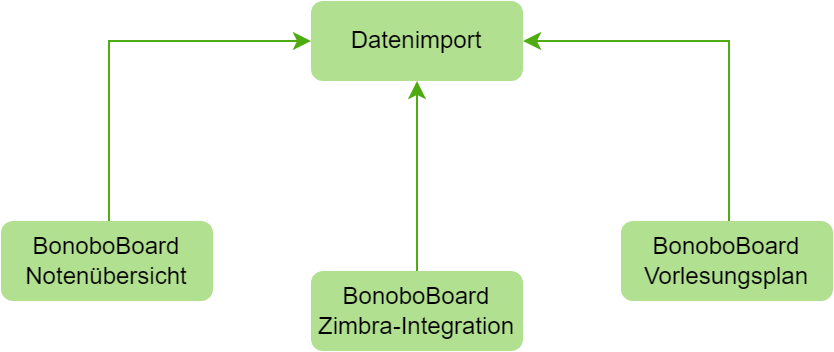
\includegraphics[width=0.8\textwidth]{Dependencies}
\caption{Projekt Abhängigkeiten}
\label{img:Dependencies}
\end{center}
\end{figure}

Das BonoboBoard umfasst vier Features, von denen eines Voraussetzung für die anderen drei ist (vgl. Abb. \ref{img:Dependencies}). Bei dem ersten handelt es sich um eine Importfunktion, die die Anmeldedaten einer Student*in für das DHBW Rechenzentrum entgegennimmt und diese nutzt, um Zugriff auf die vier wesentlichen DHBW Onlinedienste zu erhalten: Vorlesungsplan, Moodle, Dualis und Zimbra-Webclient. Mit den von diesen Onlineportalen erhaltenen Informationen werden drei Funktionen des BonoboBoards bereitgestellt: Vorlesungsplan, Notenübersicht und Mailservice.\\
Im Vorlesungsplan werden Termine und Zeiten der Veranstaltungen angezeigt und im Falle von Onlinelehre mit einem Link zu einem Online-Vorlesungsraum versehen. Diese Links werden aus dem Moodle System bezogen.\\
Die Notenübersicht zeigt der Student*in eine Leistungsübersicht an, die aus dem Dualis bezogen wird. Die Noten werden erst auf Anfrage angezeigt.\\
Der Mailservice befähigt die Student*in Emails zu lesen, zu schreiben und zu beantworten. Diese Funktionen werden unter Verwendung des Zimbra-Webclients zur Verfügung gestellt.\\
Das Tool fasst die wesentlichen Funktionen, der von der DHBW Mannheim verwendeten Onlineportalen, zentral an einer Stelle zusammen.


		%------------------------------------------------------------
		%-----  -----  ------ End actual content ------  -----  -----
		%------------------------------------------------------------
\end{document}

























